\documentclass[fontsize=11pt]{scrartcl}
\usepackage[T1]{fontenc}
\usepackage{fourier}

\usepackage[english]{babel}                                                         % English language/hyphenation
\usepackage[protrusion=true,expansion=true]{microtype}  
\usepackage{amsmath,amsfonts,amsthm} % Math packages
\usepackage[pdftex]{graphicx}   
\usepackage[hidelinks]{hyperref}
\usepackage{listings}


%%% Custom sectioning
\usepackage{sectsty}
\allsectionsfont{\centering \normalfont\scshape}


%%% Custom headers/footers (fancyhdr package)
\usepackage{fancyhdr}
\pagestyle{fancyplain}
\fancyhead{}                                            % No page header
\fancyfoot[L]{}                                         % Empty 
\fancyfoot[C]{}                                         % Empty
\fancyfoot[R]{\thepage}                                 % Pagenumbering
\renewcommand{\headrulewidth}{0pt}          % Remove header underlines
\renewcommand{\footrulewidth}{0pt}              % Remove footer underlines
\setlength{\headheight}{13.6pt}


%%% Equation and float numbering
\numberwithin{equation}{section}        % Equationnumbering: section.eq#
\numberwithin{figure}{section}          % Figurenumbering: section.fig#
\numberwithin{table}{section}               % Tablenumbering: section.tab#


%%% Maketitle metadata
\newcommand{\horrule}[1]{\rule{\linewidth}{#1}}     % Horizontal rule

\title{
        %\vspace{-1in}  
        \usefont{OT1}{bch}{b}{n}
        \horrule{0.5pt} \\[0.4cm]
        \huge Optimizing Single Core Matrix Multiply \\
        \horrule{2pt} \\[0.5cm]
}
\author{
        \normalfont                                 \normalsize
        Calvin Wylie (cjw278@cornell.edu)\\[-3pt]      \normalsize
        \today
}
\date{}


%%% Begin document
\begin{document}

\maketitle

\section{Introduction}
Matrix multiplication is a ubiquitous operation in science and engineering,
and thus the efficient and fast computation of matrix products is essential.
This report will investigate the tuning of serial matrix multiplication with the 
Intel C++ compiler (icc)\footnote{\url{https://software.intel.com/en-us/c-compilers/ipsxe}}.

Specifically, throughout this report, we will consider the problem of computing
$C = C + A B$, where $C, A, B$ are $M \times M$ square matrices.

\subsection{Testing specs}

We time the matrix multiplication routines on a single core of an Intel Xeon
E5-2620 v3 processor\footnote{\url{http://ark.intel.com/products/83352/Intel-Xeon-Processor-E5-2620-v3-15M-Cache-2_40-GHz}}.  Relavent specs for our purposes is a 256 kB L2 cache,
and 256 bit wide vector registers.

\subsection{Reference Implementations}

Our reference implementations are OpenBLAS\footnote{\url{http://www.openblas.net/}},
the Intel Math Kernel Library\footnote{\url{https://software.intel.com/en-us/intel-mkl}}, 
and the Fortran implementation fdgemm.f, which in the timing plots produced are
referred to as blas, mkl, and f2c respectively.

\subsection{Optimization}

The basic, `naive', matrix multiplication routine is a set of three nested loops, 
with code given below.

\begin{lstlisting}[frame = single, caption={Naive Square Matrix Multiply}]
void square_dgemm(const int M, 
                  const double *A, const double *B, double *C)
{
    for (int i = 0; i < M; ++i) {
        for (int j = 0; j < M; ++j) {
            for (int k = 0; k < M; ++k) {
                C[j*M+i] += A[k*M+i] * B[j*M+k];
            }
        }
    }
}
\end{lstlisting}

Timing results for this basic approach are compared against mkl, blas, and f2c
in Figure~\ref{fig:initial}. As can be seen, the naive approach is an order of 
magnitude slower than the fastest routine (mkl).  Our goal is to reorganize this
basic computation to take advantage of the features of the Xeon E5-2620, in order
to realize large performance gains.

\begin{figure}[h]
    \centering
    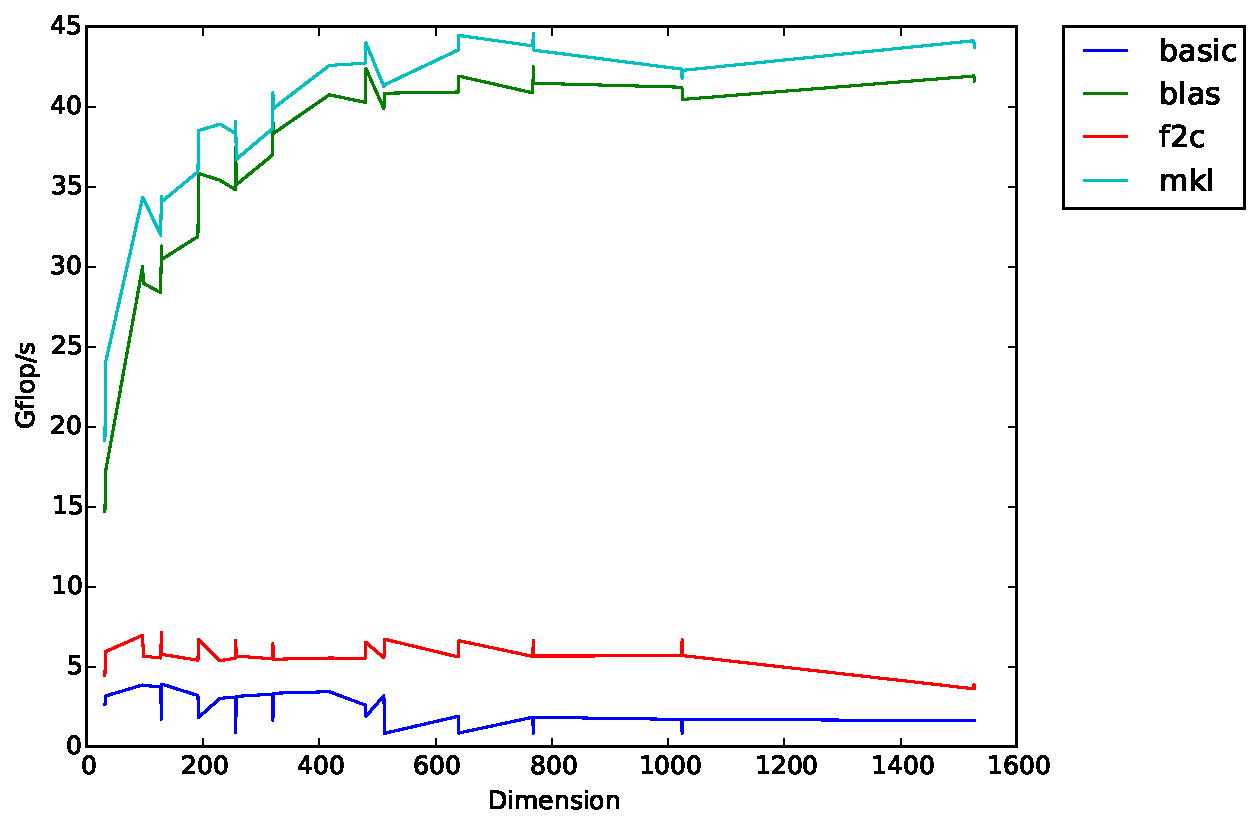
\includegraphics[width=5.0in]{../final_timings/timing_initial.pdf}
    \caption{Initial timing plot.}
    \label{fig:initial}
\end{figure}


\section{Optimization strategies}

\subsection{Putting the Compiler to Work}

We use the -O3 and the -xCORE-AVX2 optimization flags.  -xCORE-AVX2 tells the 
compiler to generate instructions optimized for our Xeon E5-2620 processor.  
However, -xCORE-AVX2 is not a ``magic'' flag that will always result in
performance gains.  Using the flag on basic matrix multiply results in no
significant performance gains (see Figure~\ref{fig:avx2}).  In order for these
optimized instructions to be effective, we need to vectorize our code.

\begin{figure}[h]
    \centering
    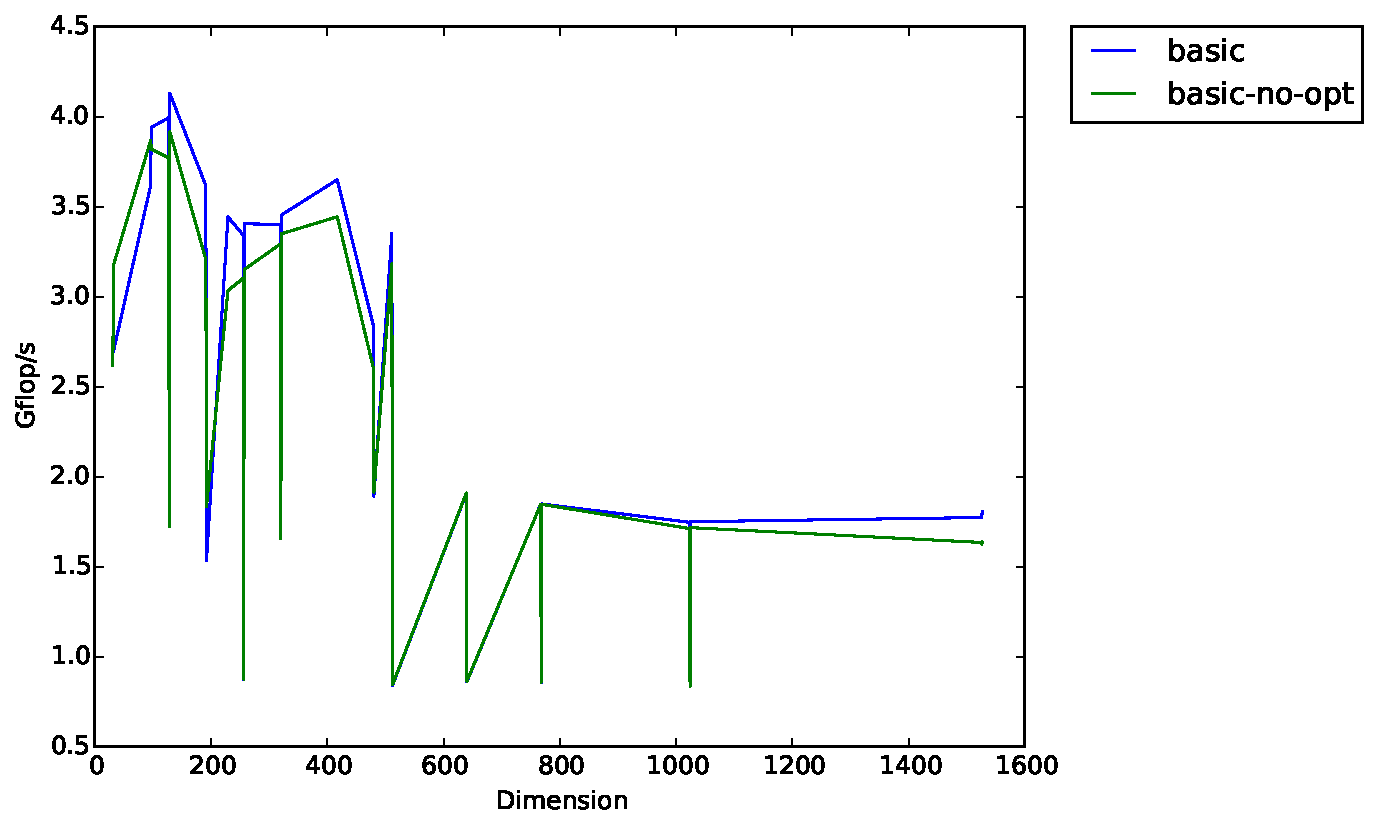
\includegraphics[width=5.0in]{../final_timings/timing_basic_avx2.pdf}
    \caption{Basic matrix multiply (basic-no-opt) compared against basic matrix multiply compiled with the -xCORE-AVX2 flag (basic).}
    \label{fig:avx2}
\end{figure}

We made extensive use of the Intel compiler optimization reports to guide our
tuning (one such report for our final matrix multiply routine can be found in
dgemm\_mine.optrpt).  Letting the compiler perform micro optimizations such as 
loop unrolling and inlining allowed us to focus on higher level optimizations such
as memory layout.  We also made use of these reports to write our code so that
the compiler could ``autovectorize'' (discussed in a later section).
dgemm\_mine.optrpt indicates that the compiler did vectorize our code, as well as
inlining all function calls and some loop unrolling.

\subsection{Regularizing Memory access}
Notice that in the naive matrix multiply implementation, the order of the loops
is arbitrary, as all computation is performed in the innermost loop.
Noting this, we can choose a loop order that best regularizes memory access.
Ideally, we would like to access the arrays with stride 1, and this motivates the
idea that the `i' variable in the naive code should be the loop index of the
innermost loop, as then we are accessing arrays C and A with stride one.  
This results in the following code:

\begin{lstlisting}[frame = single, caption={Improved Loop Order Square Matrix Multiply}]
void square dgemm(const int M, 
                  const double *A, const double *B, double *C)
{
    for (int j = 0; j < M; ++j) {
        for (int k = 0; k < M; ++k) {
            double bkj = B[j*M+k];
            for (int i = 0; i < M; ++i)
                C[j*M+i] += A[k*M+i] * bkj;
        }
    }
}
\end{lstlisting}

This optimization is supported empirically, as all possible loop orders were
tested and the results seen in Figure~\ref{fig:loop_order}).

This basic optimization brings the naive matrix multiple up to the speed of
the Fortran reference code (see Figure~\ref{fig:loop_jki}). Throughout the rest 
of this paper, we shall refer to this as the optimized (matrix multiply) kernel.

\begin{figure}[h]
    \centering
    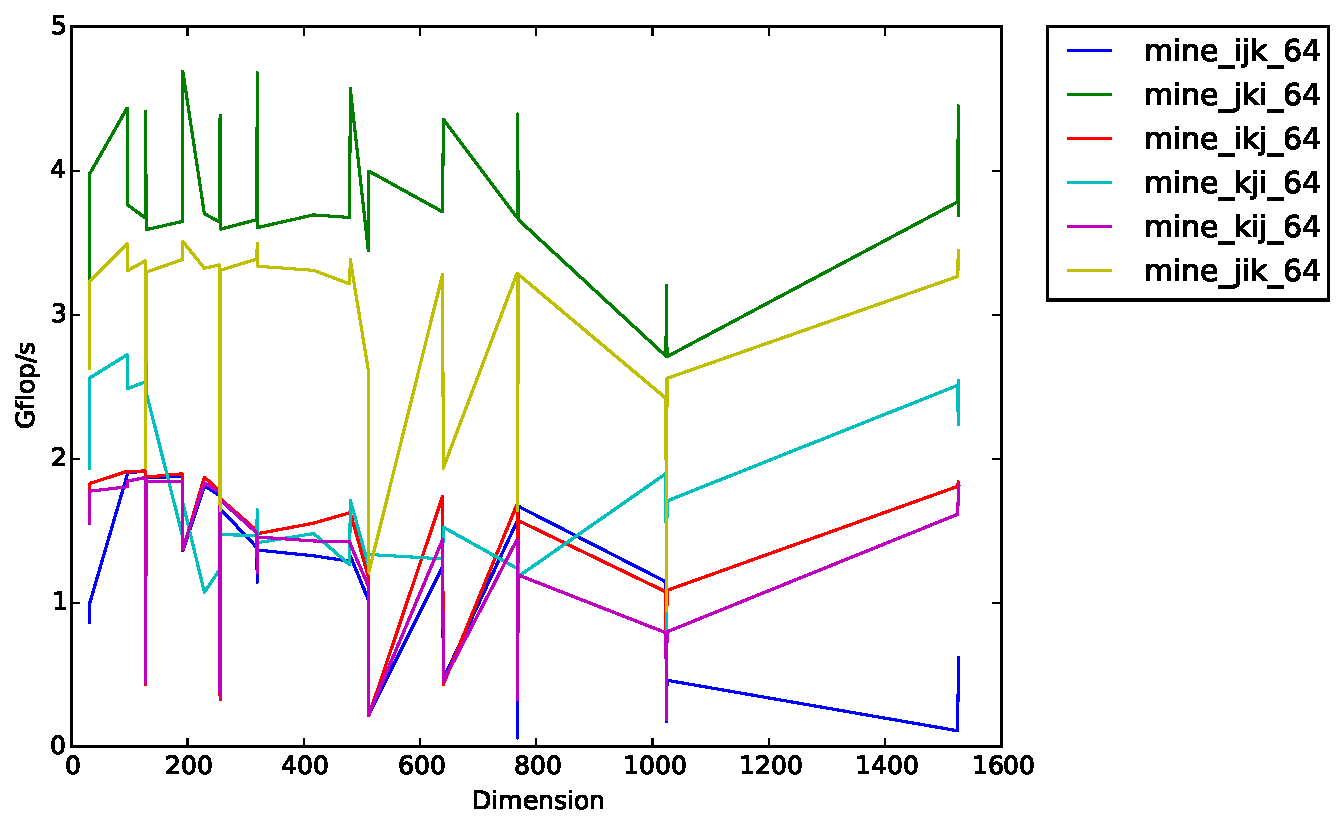
\includegraphics[width=5.0in]{../final_timings/timing_loop_order.pdf}
    \caption{Timing results for all possible loop orders.}
    \label{fig:loop_order}
\end{figure}

\begin{figure}[h]
    \centering
    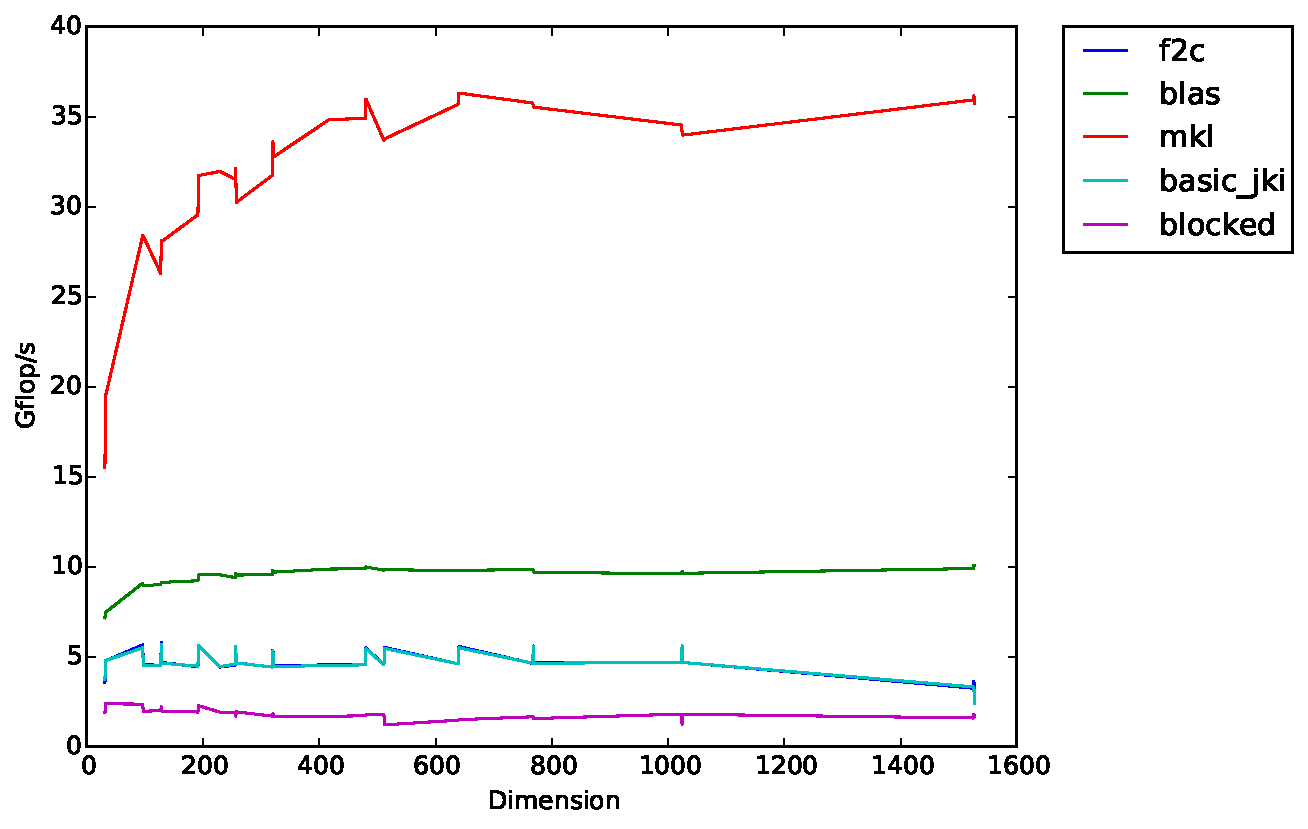
\includegraphics[width=5.0in]{../final_timings/timing_jki_compare.pdf}
    \caption{Loop order optimization comparison.}
    \label{fig:loop_jki}
\end{figure}

\subsection{Cache Reuse}
Memory accesses can be a significant source of slowdown in numerical computations.
We would like to minimize the number of times a piece of data must be loaded from
main memory, rather than from the much faster CPU cache.  One strategy for matrix
multiply that makes effective use of the CPU cache is ``blocking'', where the 
matrices $A$ and $B$ are partitioned into sub-matrices, which can be independently
multiplied together to calculate a partial result of the corresponding submatrix
$C$.  The idea is illustrated below.

\[\left( \begin{array}{cc}
C_{11} & C_{12} \\
C_{21} & C_{22} \end{array} \right)
= \left( \begin{array}{cc}
A_{11} B_{11} + A_{12} B_{21} & A_{11} B_{12} + A_{12} B_{22} \\
A_{21} B_{11} + A_{22} B_{21} & A_{21} B_{12} + A_{22} B_{22} \end{array} \right)
= \left( \begin{array}{cc}
A_{11} & A_{12} \\
A_{21} & A_{22} \end{array} \right)
\left( \begin{array}{cc}
B_{11} & B_{12} \\
B_{21} & B_{22} \end{array} \right)
\] 

We will get effective cache reuse if we choose the size of the sub-matrices so that
three of them can fit into cache simultaneously.

On the Xeon E5-2620 processor, the size of the L2 cache is 256 kB.  This motivates 
choosing a sub-matrix size of $104 \times 104$, since each double precision floating
point entry is 8 bytes.

We test various block sizes nearby $104 \times 104$ to verify that this is the best
sub-matrix size (Figure~\ref{fig:block_size}).  As seen in the results,
$104 \times 104$ is indeed the best performing block size for large dimension.

\begin{figure}[h]
    \centering
    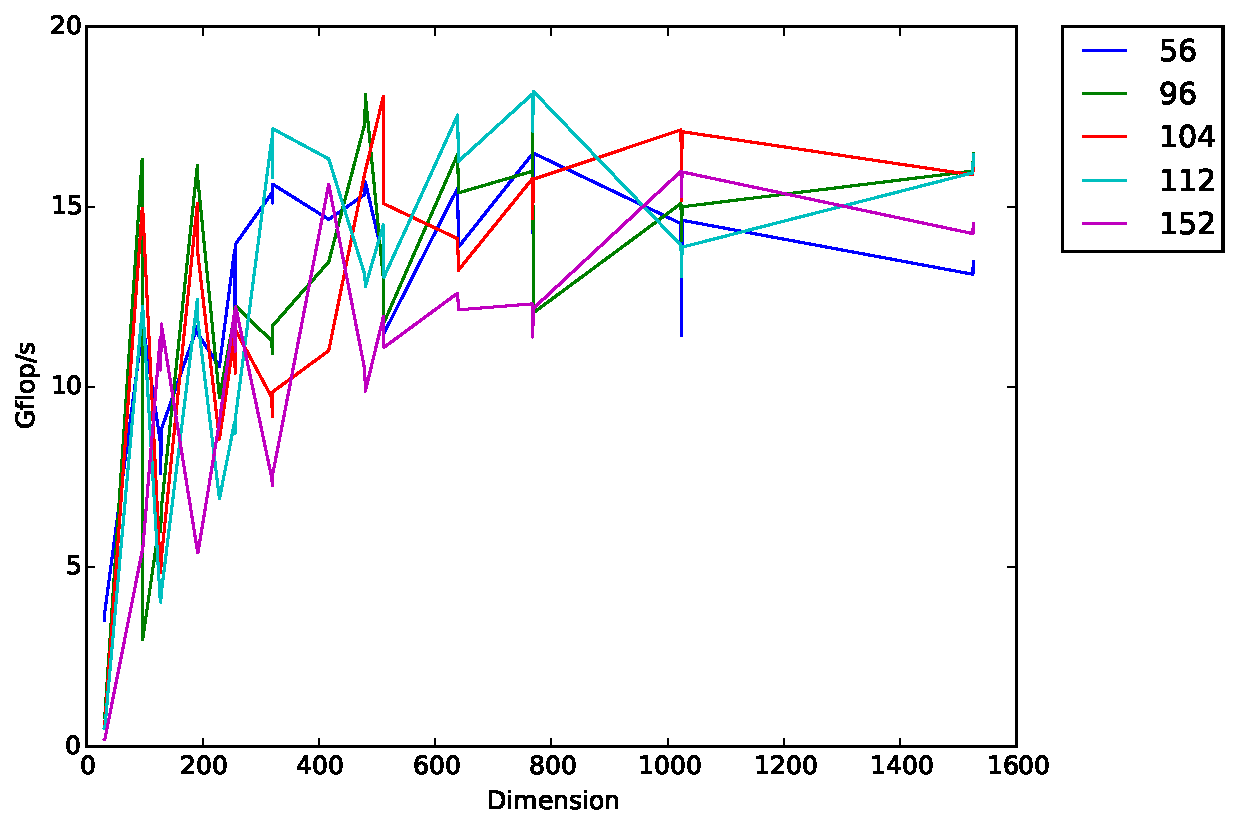
\includegraphics[width=5.0in]{../final_timings/timing_block_size.pdf}
    \caption{Sub-matrix size comparison.}
    \label{fig:block_size}
\end{figure}

For our implementation, we statically allocate three ``working'' arrays of size
$104 \times 104$.  We then loop over block combinations, load the sub-matrices 
into our working arrays, then multiply these arrays with our optimized kernel.
We then write the result back to the appropriate area of our result matrix $C$.

\subsection{Vectorization}
Another source of significant performance gains can be obtained by vectorization.
Vectorization is ``the untrolling of a loop combined with [...] SIMD instructions''
\footnote{\url{https://software.intel.com/sites/default/files/m/4/8/8/2/a/31848-CompilerAutovectorizationGuide.pdf}}.

We decided that rather than attempt to write SSE/AVX instructions by hand, we 
would rely on the autovectorization capabilities of the Intel compiler.

To assist the Intel compiler in autovectorization, we align our working arrays
to 64 byte boundaries (since the AVX2 instruction set operates most efficiently
on 64 byte aligned data), as well as make use of the `restrict' keyword 
(and -restrict compiler flag), indicating that the pointers to our data do not 
overlap.  See the previously linked Intel guide for more in depth rationale 
behind these compile time optimizations.

Since the vector registers are 256 bits wide (4 double precision floating point 
numbers), we employ a multi-level blocking strategy, where our copied sub-matrix 
blocks are further subdivided into $4 \times 4$ matrix product calculations 
(though unlike in the initial blocking strategy, we do not copy these 
sub-sub-matrices into new memory locations).

\subsection{Final Results}

Our final code can be seen in dgemm\_mine.c. The final results after performing 
all the above optimizations can be seen in Figure~\ref{fig:final}.  
Notice the significant performance gain over the basic
matrix multiply routine.  We achieve a peak performance of roughly 18 Gflops/s, 
which is roughly 40 per cent of the peak performance of the Intel Math Kernel
Library.

\begin{figure}[h]
    \centering
    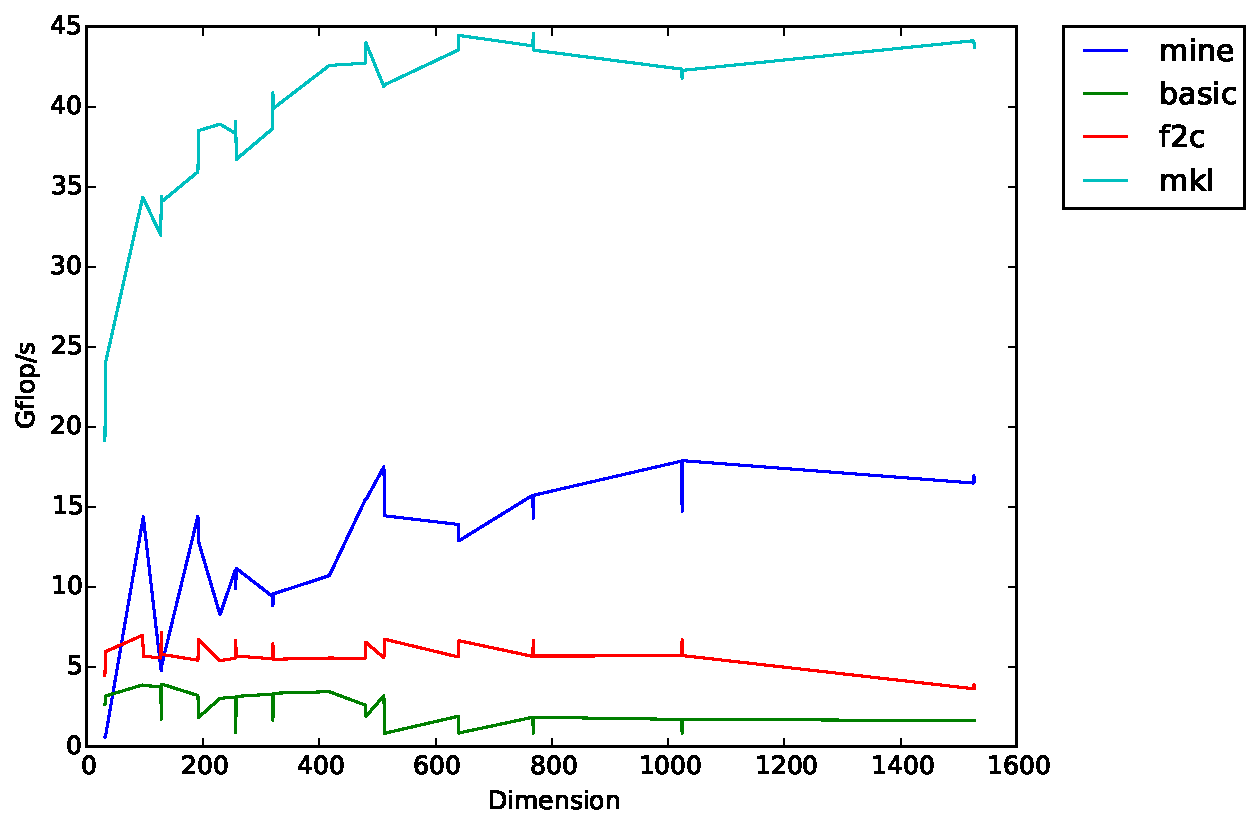
\includegraphics[width=5.0in]{../final_timings/timing_104_4.pdf}
    \caption{Final optimized code timing comparison.}
    \label{fig:final}
\end{figure}

\section{Future Work}

Below we briefly dicuss some possible directions to further optimize our
matrix multiply routine.

\subsection{Automated Tuning}
One beneficial tool would be an ``automated tuner'', a script that could 
search over the complete space of parameterizations (loop order, block size, etc.)
to identify the optimal parameterization.

\subsection{Kernel Tuning}
Rather than relying on the autovectorization capabilities of the Intel compiler,
we could instead hand code the SSE/AVX instructions for our kernel.  Done 
correctly this would likely lead to performance gains, as we would have direct
control over the instructions generated by the compiler.

\end{document}